% Part 2 chapter carrying "The Baryon Asymmetry as a Derived Quantity: CMB Evidence Without BBN Prior" (March 2026) line for line
% (PDF read in full 2026-10-03: 242 text lines, 50-line ledger, no gaps; LaTeX docs/papers/latex/Evidence_Baryon for equation forms),
% section 8 of "Matter-Antimatter Asymmetry and the Information Writing Constraint" (the same chain), and the 18th-chain record
% docs/papers/18thChainBaryonAsymmetry.rtf (7 RTF lines; text read in full). Chain settings from
% mgcamb_validation/yaml_configs/iam_baryon_test.updated.yaml.
% Corrections: PAPER_ERRATA C3, C4, C6-C12, C22, C23; CC_AND_BARYON_CHECK.md items 1-5, 22-24. C10 traced here: Cyburt et al. 2016
% Table IV has no 6.137 +/- 0.017; the comparators are now the values printed in that table and in Planck 2018 VI Table 2.
% Numbers: docs/verification/scripts/verify_lambda_baryon_book.py, sections E, F.
\chapter{The baryon density from the microwave background alone}\label{ch:baryon_chain}

The baryon-to-photon ratio $\eta\approx6.1\times10^{-10}$ is conventionally a free parameter, measured independently by nucleosynthesis
and by the CMB acoustic peaks but not derived from a deeper principle. Chapter~\ref{ch:baryon} set out a self-consistency constraint that
would connect $\eta$ to the universe's information-writing budget: the same law that reads the cosmological constant as the accumulated
Landauer cost of baryonic decoherence (Chapter~\ref{ch:lambda}) would require a specific baryon density. \conjecture\ This chapter
carries the chain that was run to look at it: the Planck 2018 CMB likelihood with $\Omega_bh^2$ sampled over a flat range six times wider
than in the other runs, and no light-element abundance data. The posterior is $\eta=(6.113\pm0.037)\times10^{-10}$. \measured\ It is the
value every CMB fit returns, and the chapter states what that does and does not show.

\section{Two measured numbers}\label{sec:bc_intro}
The baryon-to-photon ratio,
\begin{equation}\eta\equiv\frac{n_b-n_{\bar b}}{n_\gamma}\approx6.1\times10^{-10},\label{eq:bc_eta}\end{equation}
is one of the most precisely measured dimensionless numbers in cosmology, determined independently by the light-element abundances of
Big Bang nucleosynthesis~\cite{Cyburt2016} and by the CMB acoustic peaks~\cite{Planck2018VI}. Both measurements agree. \observed\ Neither explains
why $\eta$ has this value. In the standard framework $\eta$ is a free parameter fixed by baryogenesis dynamics whose output depends on
model-specific parameters not derived from first principles~\cite{RubakovShaposhnikov1996,Davidson2008}.

The cosmological constant is in an analogous position. Its observed value is known precisely but lies about 123 orders of magnitude below
the naive quantum-field-theory vacuum energy (Chapter~\ref{ch:lambda}). Both $\eta$ and $\Lambda$ are measured with precision and not
explained. \observed

IAM's Law proposes that both are set by the same constraint. Every irreversible crossing from a quantum superposition to a classical
record pays a thermodynamic cost to the nearest encoding surface,
\begin{equation}\Delta E_{\rm act}=k_BT_H\ln2\quad\text{per bit}\label{eq:bc_law}\end{equation}
(Chapter~\ref{ch:iams_law}). \derived\ (Landauer's bound at the surface temperature) Applied over cosmic history, the law reads
$\Lambda_{\rm obs}$ as the accumulated Landauer cost of baryonic decoherence. The accumulated cost depends directly on $\Omega_b$, which
$\eta$ sets before nucleosynthesis, so the law connects $\Lambda$ and $\eta$ through the information-writing budget: the universe could
sustain only the baryon density at which the Landauer cost matches the observed dark-energy density. \conjecture

Before the chain was run, the expectation was stated that a chain with $\Omega_bh^2$ free would return a posterior consistent with
$\eta\approx6\times10^{-10}$ from CMB data alone. Because the informational term is off at recombination, every CMB fit returns that
value (Section~\ref{sec:bc_result}), so the run is a consistency check on the informational term, not an independent test of it. \interp

\section{The constraint in terms of $\Omega_b$}\label{sec:bc_constraint}
The cosmological-constant expression of Chapter~\ref{ch:lambda} is
\begin{equation}\frac{\rho_\Lambda}{\rho_{\rm vac}}=\frac{2}{\pi}\left(\frac{l_P}{l_H}\right)^2\frac{\Omega_b}{\Omega_m},\label{eq:bc_cc}\end{equation}
with $l_P$ the Planck length, $l_H$ the Hubble length and $\Omega_b/\Omega_m$ the baryonic fraction of matter (Eq.~\eqref{eq:base};
the coefficient $2/\pi$ is taken as given here; its derivation is an open problem, Section~\ref{sec:lam_twopi}). \openprob\ The departure from exact de Sitter geometry was taken to
introduce the ratio of the Gibbons--Hawking temperatures of the de Sitter encoding surface and the Hubble writing temperature,
\begin{equation}\frac{T_{dS}}{T_H}=\frac{H_{dS}}{H_0}=\sqrt{\Omega_\Lambda},\label{eq:bc_tratio}\end{equation}
\derived\ (the temperature of the horizon set by $\Lambda$ alone) and with it
\begin{equation}\frac{\rho_\Lambda}{\rho_{\rm vac}}\bigg|_{T_{dS}}=\frac{2}{\pi}\left(\frac{l_P}{l_H}\right)^2\sqrt{\Omega_\Lambda}\,
\frac{\Omega_b}{\Omega_m}=1.142\times10^{-123}\label{eq:bc_cccorr}\end{equation}
against the observed $1.133\times10^{-123}$, $0.79\,\%$ above it (Eq.~\eqref{eq:corr}). \fitted\ The expression contains $\Omega_b$
explicitly. Inverting it --- asking what $\Omega_b$ the observed $\Lambda$ requires --- gives a value of $\Omega_bh^2$, and so of $\eta$
through~\cite{Steigman2006}
\begin{equation}\eta=2.739\times10^{-8}\,\Omega_bh^2 .\label{eq:bc_etaob}\end{equation}
\derived\ With Planck 2018 central values ($\Omega_mh^2=0.1431$, $\Omega_\Lambda=0.6847$~\cite{Planck2018VI}), Eq.~\eqref{eq:bc_cc}
inverted gives $\Omega_bh^2=0.01837$ and $\eta=5.03\times10^{-10}$, and Eq.~\eqref{eq:bc_cccorr} inverted gives $\Omega_bh^2=0.02220$ and
$\eta=6.08\times10^{-10}$. \calc\ The second is $0.8\,\%$ below the Planck value $6.127$; it is the relation
$\Omega_b/\Omega_m=\tfrac3{16}\sqrt{\Omega_\Lambda}$ (Eq.~\eqref{eq:rel}) read in the variable $\eta$, not a separate result.

\section{The chain}\label{sec:bc_chain}
\subsection{Setup}
The chain uses the configuration of the Level~1 runs (Chapter~\ref{ch:dual}): MGCAMB~\cite{Zhao2009MGCAMB,Wang2023MGCAMB} on CAMB
1.5.2~\cite{Lewis2000CAMB} with Cobaya 3.6~\cite{Torrado2021}, the Planck 2018 likelihoods low-$\ell$ TT, low-$\ell$ EE, high-$\ell$
plik TTTEEE lite (native) and CMB lensing~\cite{Planck2018V,Planck2018VIII}, and the informational term fixed at $\mu_0=-0.13495$
(Chapter~\ref{ch:theory}). All standard parameters are sampled; the reference values in Table~\ref{tab:bc_yaml} are the distributions the
walkers start from, not priors. The one change from the other runs is the range of $\Omega_bh^2$:
\begin{align}
\text{other runs:}\quad &\Omega_bh^2\ \text{flat on }[0.020,\,0.025],\quad \text{start }\mathcal N(0.02242,\,0.00014^2),\label{eq:bc_std}\\
\text{this chain:}\quad &\Omega_bh^2\ \text{flat on }[0.010,\,0.040],\quad \text{start }\mathcal N(0.02242,\,0.001^2).\label{eq:bc_test}
\end{align}
The range is six times wider ($0.030$ against $0.005$). \calc\ Neither setting is a nucleosynthesis prior: the narrow normal is Cobaya's
starting distribution, and the prior in every run is flat. The chain uses no light-element abundance data, no BAO, no supernovae and no
$H_0$ prior. Helium is not sampled or fixed, so CAMB sets $Y_{\rm He}$ from $\Omega_bh^2$ by its standard nucleosynthesis consistency
relation, as in the Planck analyses; nuclear physics enters only through the helium fraction in the damping tail, not as a constraint on
$\Omega_bh^2$. \observed\ The walkers start at the same place; the chain is free to move to a different $\Omega_bh^2$ if the CMB data prefer
one.

\begin{table}[htbp]\centering\small
\caption[Settings of the 18th chain]{Settings of the 18th chain, from \texttt{mgcamb\_validation/\allowbreak{}yaml\_configs/\allowbreak{}iam\_baryon\_test.updated.yaml}. Priors are flat unless stated; ``start'' is the reference distribution from which the walkers begin.}\label{tab:bc_yaml}
\begin{tabular}{llll}\toprule
Parameter & Prior & Start & Proposal\\\midrule
$\Omega_bh^2$ & $[0.010,\,0.040]$ & $\mathcal N(0.02242,\,0.001)$ & 0.001\\
$\Omega_ch^2$ & $[0.10,\,0.14]$ & $\mathcal N(0.11933,\,0.00091)$ & 0.00091\\
$H_0$ & $[60,\,80]$ & $\mathcal N(67.4,\,0.5)$ & 0.5\\
$\tau$ & $[0.01,\,0.12]$ & $\mathcal N(0.0544,\,0.0073)$ & 0.0073\\
$\ln(10^{10}A_s)$ & $[2.6,\,3.5]$ & $\mathcal N(3.044,\,0.014)$ & 0.014\\
$n_s$ & $[0.92,\,1.00]$ & $\mathcal N(0.9649,\,0.0042)$ & 0.0042\\
$A_{\rm Planck}$ & $\mathcal N(1,\,0.0025)$ & $\mathcal N(1,\,0.002)$ & 0.0005\\
$\mu_0$ & fixed $-0.13495$ & --- & ---\\
$Y_{\rm He}$ & from $\Omega_bh^2$ (CAMB) & --- & ---\\\midrule
Stop & \multicolumn{3}{l}{$R-1<0.01$ (means), $R-1<0.15$ (95\,\% bounds)}\\\bottomrule
\end{tabular}
\end{table}

\subsection{Run and convergence}
The chain ran from 19 March 2026, 22:52, to 20 March 2026, 04:35. The run log records the last convergence tests:
\begin{table}[htbp]\centering\small
\caption[Convergence of the 18th chain]{The last convergence tests of the 18th chain, from its run log. $R-1$ is the Gelman--Rubin statistic of the means over the last part of the chain.}\label{tab:bc_conv}
\begin{tabular}{rrl}\toprule
Accepted samples at test & $R-1$ (means) & over the last\\\midrule
(21{,}560)$^{a}$ & 0.012617 & 17{,}248 \\
21{,}840 & 0.011284 & 17{,}472 \\
22{,}120 & 0.009664 & 17{,}696 \\
22{,}400 & 0.009273 & 17{,}920 \\\midrule
\multicolumn{3}{l}{At 22,400: $R-1$ of the bounds 0.063629; acceptance rate 0.749; sampling complete.}\\
\multicolumn{3}{l}{$^{a}$ The log shows only the result line; $17{,}248/0.8$.}\\\bottomrule
\end{tabular}
\end{table}
\measured\ The chain file holds 21,366 rows; with 30\,\% burn-in, 14,957. \observed\

\subsection{Result}\label{sec:bc_result}
With 30\,\% burn-in the weighted posterior is
\begin{equation}\Omega_bh^2=0.022320\pm0.000136,\label{eq:bc_ob}\end{equation}
which by Eq.~\eqref{eq:bc_etaob} is
\begin{equation}\eta=(6.113\pm0.037)\times10^{-10}.\label{eq:bc_etares}\end{equation}
\measured\ The record of the run gives $\Omega_bh^2=0.022319\pm0.000136$ and $\eta=6.1155\times10^{-10}$; the difference in $\eta$ is
the conversion factor ($2.74\times10^{-8}$ in the record, $2.739\times10^{-8}$ here), not the burn-in. \calc\ The $\Omega_bh^2$
posterior is single-peaked and Gaussian with no multimodality, and stays between $0.0218$ and $0.0228$ although the range allowed is
$0.010$--$0.040$ (Fig.~\ref{fig:baryon_posterior}). \measured\ The same chain gives $H_0=67.04\pm0.53$, $\Omega_m=0.3198\pm0.0075$,
$\Omega_b/\Omega_m=0.1554\pm0.0019$, and the ratio of the two sides of Eq.~\eqref{eq:rel}
\begin{equation}\frac{\Omega_b/\Omega_m}{(3/16)\sqrt{\Omega_\Lambda}}=1.0046\pm0.0068\quad(0.7\sigma).\label{eq:bc_ratio}\end{equation}
\measured

\begin{figure}[htbp]\centering
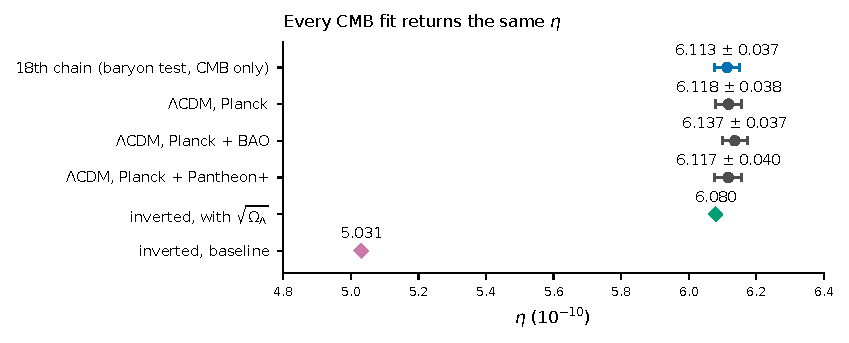
\includegraphics[width=0.75\textwidth]{figures/part2/fig_eta.pdf}
\caption{$\eta=273.9\times10^{-10}\,\Omega_bh^2$ on the 18th chain ($6.113\pm0.037$) and on the $\Lambda$CDM chains ($6.117$--$6.137$): every CMB fit returns the same baryon density \observed. Diamonds: the cosmological-constant expressions inverted for $\Omega_bh^2$ at $\Omega_mh^2=0.1431$, 6.080 with $\sqrt{\Omega_\Lambda}$ and 5.031 without; this is the relation of Fig.~\ref{fig:cc_relation} in another variable. \calc}\label{fig:eta}
\end{figure}

\section{What the chain shows}\label{sec:bc_interp}
Table~\ref{tab:bc_compare} sets the chain beside the measured values and the inverted expression.
\begin{table}[htbp]\centering\small
\caption[The baryon-to-photon ratio from each source]{The baryon-to-photon ratio from each source, in units of $10^{-10}$. Measured values as printed in the sources; Planck values converted with Eq.~\eqref{eq:bc_etaob}.}\label{tab:bc_compare}
\begin{tabularx}{\linewidth}{>{\raggedright\arraybackslash}Xlll}\toprule
Source & $10^{10}\eta$ & Method & Label\\\midrule
Nucleosynthesis with deuterium~\cite{Cyburt2016} (Table IV) & $6.180\pm0.195$ & light-element abundances & \measured\\
CMB only, same analysis~\cite{Cyburt2016} (Table IV) & $6.108\pm0.060$ & acoustic peaks & \measured\\
CMB + nucleosynthesis~\cite{Cyburt2016} (Table IV) & $6.098\pm0.042$ & combined & \measured\\
Planck 2018 TT,TE,EE+lowE+lensing~\cite{Planck2018VI} & $6.127\pm0.041$ & acoustic peaks & \measured\\
Planck 2018 + BAO~\cite{Planck2018VI} & $6.141\pm0.038$ & acoustic peaks + BAO & \measured\\
18th chain (this chapter) & $6.113\pm0.037$ & CMB only, flat range 0.010--0.040 & \measured\\
Expression \eqref{eq:bc_cccorr} inverted & $6.080$ & $\Omega_b/\Omega_m=\tfrac3{16}\sqrt{\Omega_\Lambda}$ & \calc\\
Expression \eqref{eq:bc_cc} inverted & $5.031$ & $\Omega_b/\Omega_m=\tfrac3{16}\Omega_\Lambda$ & \calc\\\bottomrule
\end{tabularx}
\end{table}

The chain agrees with nucleosynthesis ($6.113$ against $6.180\pm0.195$, $0.3\sigma$) and with Planck ($0.2\,\%$ below $6.127$).
\calc\ That agreement is the established CMB--nucleosynthesis concordance~\cite{Cyburt2016,Planck2018VI}: the CMB measures $\Omega_bh^2$
from the baryon loading of the photon--baryon fluid at recombination, imprinted on the relative heights of the acoustic peaks, and
nucleosynthesis measures it from the abundance ratios of the light elements through the nuclear reaction network. These are two
independent measurements of one number. \observed

The chain contains no constraint from the cosmological-constant expression: Eq.~\eqref{eq:bc_cccorr} is not in its likelihood, and fixing
$\mu_0$ or widening the range does not move $\Omega_bh^2$. The $\Lambda$CDM chains in the same repository give the same value
(Table~\ref{tab:baryon_chains}). They must: the informational term is off at recombination ($E\to0$), so IAM's own equations reproduce the $\Lambda$CDM early universe with no added parameter, and the acoustic peaks return the measured baryon density with the term in place. The chain is the consistency check that the term
leaves the early universe intact, and it passes. \observed\ What it adds is the relation of Chapter~\ref{ch:lambda} evaluated on a
CMB-only posterior: $1.0046\pm0.0068$, $0.7\sigma$ (Eq.~\eqref{eq:bc_ratio}). \measured

\begin{table}[htbp]\centering\small
\caption[The baryon density on every chain]{The baryon density on every chain, $\eta=273.9\times10^{-10}\,\Omega_bh^2$ (30\,\% burn-in, weighted mean and standard deviation; rows after burn-in), and the cosmological-constant expressions inverted for $\Omega_bh^2$ at the Planck $\Omega_mh^2=0.1431$.}\label{tab:baryon_chains}
\begin{adjustbox}{max width=\textwidth}
\begin{tabular}{lcrccll}\toprule
Source & $\Omega_bh^2$ range & rows & $\Omega_bh^2$ & $10^{10}\eta$ & ratio to $(3/16)\sqrt{\Omega_\Lambda}$ & Label\\\midrule
18th chain (CMB only) & 0.010--0.040 & 14{,}957 & $0.02232\pm0.00014$ & $6.113\pm0.037$ & $1.0046\pm0.0068$ & \measured\\
$\Lambda$CDM, Planck & 0.020--0.025 & 12{,}544 & $0.02234\pm0.00014$ & $6.118\pm0.038$ & $1.0058\pm0.0067$ & \measured\\
$\Lambda$CDM, Planck + BAO & 0.020--0.025 & 12{,}600 & $0.02240\pm0.00014$ & $6.137\pm0.037$ & $1.0106\pm0.0064$ & \measured\\
$\Lambda$CDM, Planck + Pantheon+ & 0.020--0.025 & 21{,}168 & $0.02233\pm0.00014$ & $6.117\pm0.040$ & $1.0056\pm0.0070$ & \measured\\
$\Lambda$CDM, Planck + BOSS DR12 $f\sigma_8$ + BAO & 0.020--0.025 & 18{,}424 & $0.02239\pm0.00014$ & $6.134\pm0.037$ & $1.0098\pm0.0062$ & \measured\\
Expression with $2/\pi$, without $\sqrt{\Omega_\Lambda}$ & --- & --- & $0.01837$ & $5.031$ & --- & \calc\\
Expression with $\sqrt{\Omega_\Lambda}$ & --- & --- & $0.02220$ & $6.080$ & --- & \calc\\\bottomrule
\end{tabular}
\end{adjustbox}
\end{table}

\begin{figure}[htbp]\centering
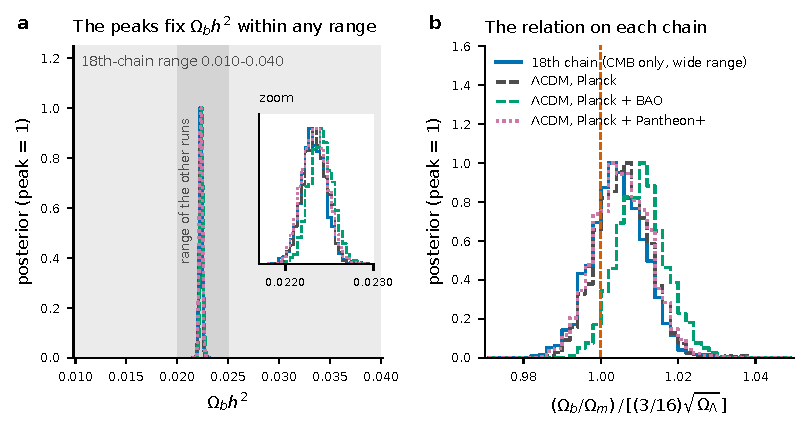
\includegraphics[width=\textwidth]{figures/part2/fig_baryon_posterior.pdf}
\caption[The 18th chain against the $\Lambda$CDM chains]{(a) The $\Omega_bh^2$ posterior of the 18th chain, sampled over the flat range 0.010--0.040 (light band; the darker band is the 0.020--0.025 of the other runs), and of three $\Lambda$CDM chains; inset: the peaks enlarged. The acoustic peaks fix $\Omega_bh^2=0.02232\pm0.00014$ whatever the range. (b) The posterior of $(\Omega_b/\Omega_m)/[(3/16)\sqrt{\Omega_\Lambda}]$ on the same chains. Chain files in \texttt{mgcamb\_validation/\allowbreak{}chains}, 30\,\% burn-in, weighted. \measured}\label{fig:baryon_posterior}
\end{figure}

\section{Falsification}\label{sec:bc_falsify}
A chain returning $\eta$ far from $6\times10^{-10}$ would have contradicted the early universe of every CMB analysis, not the loop of
Chapter~\ref{ch:baryon} specifically; it would have shown that the informational term disturbs recombination, which by construction it
does not. The chain therefore confirms consistency, not selection. The test of selection is a chain in which the writing constraint
itself is in the likelihood, so that $\Omega_b$ is predicted from $\Lambda$ rather than measured from the peaks. \openprob

The temperature ratio $\sqrt{\Omega_\Lambda}=0.827$ that brings Eq.~\eqref{eq:bc_cc} to $+0.79\,\%$ of the observed $\Lambda$ also moves
the inverted $\eta$ from $5.03$ to $6.08\times10^{-10}$, toward the chain value. These are not two corrections that agree: they are the
same relation, $\Omega_b/\Omega_m=\tfrac3{16}\sqrt{\Omega_\Lambda}$, read in two variables, and the factor was introduced to close the
first. \fitted\ The epoch-dependent history integral (Eq.~\eqref{eq:lh_integral}) is dominated by its lower limit as
written (Chapter~\ref{ch:lambda_history}); an independent derivation is the next step. \openprob

\section{Conclusions}\label{sec:bc_concl}
With $\Omega_bh^2$ free across a flat range six times wider than in the other runs and no abundance data, the Planck 2018 CMB likelihood
returns $\eta=(6.113\pm0.037)\times10^{-10}$, $0.2\,\%$ below the Planck 2018 value and $0.3\sigma$ from nucleosynthesis with
deuterium. \measured\ This is CMB--nucleosynthesis concordance, as in Planck 2018, and it shows that the informational term leaves the
early universe intact. \observed\ The constraint that would make $\eta$ a derived quantity --- the writing constraint in the likelihood,
and the coefficient $3/16$ from physics --- is the open problem. \openprob\ Within GR with the informational term, the cosmological
constant problem and the baryon-asymmetry problem are then one measured relation at the present epoch,
$\Omega_b/\Omega_m=\tfrac3{16}\sqrt{\Omega_\Lambda}$. \observed

All chains, the YAML configuration and the analysis scripts are in the repository: the chain files are
\texttt{mgcamb\_validation/\allowbreak{}chains/\allowbreak{}iam\_baryon\_test.*} (a copy in \texttt{mgcamb\_validation/}), the configuration
\texttt{mgcamb\_validation/\allowbreak{}yaml\_configs/\allowbreak{}iam\_baryon\_test.updated.yaml}, and every number of this chapter is
recomputed by \texttt{docs/verification/\allowbreak{}scripts/\allowbreak{}verify\_lambda\_baryon\_book.py}.

The chain returns the early universe that every CMB analysis returns, with the informational term in place. A cosmologist with the pipeline in Appendix~\ref{app:repro} can rerun it and take the next step: put the writing constraint itself into the likelihood.
